\documentclass[11pt]{article}
\usepackage{graphicx}
\usepackage{geometry}
\usepackage{hyperref}
\usepackage[utf8x]{inputenc}
\usepackage{footnote}
\usepackage{cite}
\usepackage{wrapfig}
\usepackage{float}

\title{P\&S SDR: Software Defined Radio\\ ETH Zurich}
\author{Philip Wiese, Sevrin Mathys, Julian Merkofer}
\date{\today}



\begin{document}

\maketitle

\thispagestyle{empty}
\vspace{12cm}
\begin{center}
	This report is licensed under CC-BY-[SA]-v4.
\end{center}

\newpage
\tableofcontents

\pagebreak
\section{Introduction}
The goal of this P\&S project is to receive the DSB\footnote{Direct Sounder Broadcast} of NOAA weather satellites. 

\section{Hardware}

\subsection{Antenna Design}
We decided to use a simple V-Dipole Antenna over a more complex QFH\footnote{Quadrifilar Helicoidal Antennas} based on the the article\cite{Adam-9A4QV:2015} of Adam.

\begin{figure}[H]
	\begin{center}
		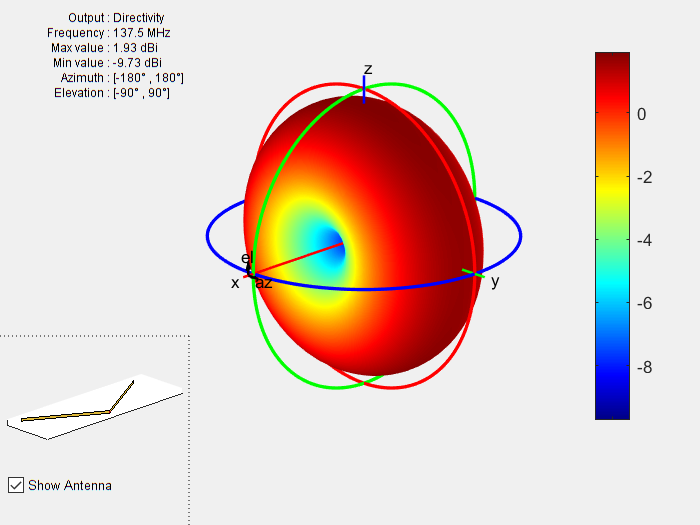
\includegraphics[scale=0.5]{img/Radiation3D.png}
		\caption{Radiation Pattern}
		\label{img_state}
	\end{center}
\end{figure}

The resonant frequency of the antenna is tuned to 137.5 MHz resulting in a leg length of 53cm. Because of the strength of the signal and the added complexity we decided not to use a Balun\footnote{\href{https://de.wikipedia.org/wiki/Balun}{www.de.wikipedia.org/wiki/Balun}}.

\subsection{Software Defined Radio}

\section{Software}
\subsection{GnuRadio}
\subsection{Python}

\section{Conclusion}


\cite{Nebarnix:2016}

\newpage

\bibliography{SDR_NOAA_Report} 
\bibliographystyle{ieeetr}

\end{document}
